%%%%%%%%%%%%%%%%%%%%%%%%%%%%%%%%%%%%%%%%%
% Wenneker Assignment
% LaTeX Template
% Version 2.0 (12/1/2019)
%
% This template originates from:
% http://www.LaTeXTemplates.com
%
% Authors:
% Vel (vel@LaTeXTemplates.com)
% Frits Wenneker
%
% License:
% CC BY-NC-SA 3.0 (http://creativecommons.org/licenses/by-nc-sa/3.0/)
% 
%%%%%%%%%%%%%%%%%%%%%%%%%%%%%%%%%%%%%%%%%

%----------------------------------------------------------------------------------------
%	PACKAGES AND OTHER DOCUMENT CONFIGURATIONS
%----------------------------------------------------------------------------------------

\documentclass[11pt]{scrartcl} % Font size

%%%%%%%%%%%%%%%%%%%%%%%%%%%%%%%%%%%%%%%%%
% Wenneker Assignment
% Structure Specification File
% Version 2.0 (12/1/2019)
%
% This template originates from:
% http://www.LaTeXTemplates.com
%
% Authors:
% Vel (vel@LaTeXTemplates.com)
% Frits Wenneker
%
% License:
% CC BY-NC-SA 3.0 (http://creativecommons.org/licenses/by-nc-sa/3.0/)
% 
%%%%%%%%%%%%%%%%%%%%%%%%%%%%%%%%%%%%%%%%%

%----------------------------------------------------------------------------------------
%	PACKAGES AND OTHER DOCUMENT CONFIGURATIONS
%----------------------------------------------------------------------------------------

\usepackage{amsmath, amsfonts, amsthm} % Math packages

\usepackage{listings} % Code listings, with syntax highlighting

\usepackage[english]{babel} % English language hyphenation

\usepackage{graphicx} % Required for inserting images
\graphicspath{{Figures/}{./}} % Specifies where to look for included images (trailing slash required)

\usepackage{booktabs} % Required for better horizontal rules in tables

\numberwithin{equation}{section} % Number equations within sections (i.e. 1.1, 1.2, 2.1, 2.2 instead of 1, 2, 3, 4)
\numberwithin{figure}{section} % Number figures within sections (i.e. 1.1, 1.2, 2.1, 2.2 instead of 1, 2, 3, 4)
\numberwithin{table}{section} % Number tables within sections (i.e. 1.1, 1.2, 2.1, 2.2 instead of 1, 2, 3, 4)

\setlength\parindent{0pt} % Removes all indentation from paragraphs

\usepackage{enumitem} % Required for list customisation
\setlist{noitemsep} % No spacing between list items

%----------------------------------------------------------------------------------------
%	DOCUMENT MARGINS
%----------------------------------------------------------------------------------------

\usepackage{geometry} % Required for adjusting page dimensions and margins

\geometry{
	paper=a4paper, % Paper size, change to letterpaper for US letter size
	top=2.5cm, % Top margin
	bottom=3cm, % Bottom margin
	left=3cm, % Left margin
	right=3cm, % Right margin
	headheight=0.75cm, % Header height
	footskip=1.5cm, % Space from the bottom margin to the baseline of the footer
	headsep=0.75cm, % Space from the top margin to the baseline of the header
	%showframe, % Uncomment to show how the type block is set on the page
}

%----------------------------------------------------------------------------------------
%	FONTS
%----------------------------------------------------------------------------------------

\usepackage[utf8]{inputenc} % Required for inputting international characters
\usepackage[T1]{fontenc} % Use 8-bit encoding

\usepackage{fourier} % Use the Adobe Utopia font for the document

%----------------------------------------------------------------------------------------
%	SECTION TITLES
%----------------------------------------------------------------------------------------

\usepackage{sectsty} % Allows customising section commands

\sectionfont{\vspace{6pt}\centering\normalfont\scshape} % \section{} styling
\subsectionfont{\normalfont\bfseries} % \subsection{} styling
\subsubsectionfont{\normalfont\itshape} % \subsubsection{} styling
\paragraphfont{\normalfont\scshape} % \paragraph{} styling

%----------------------------------------------------------------------------------------
%	HEADERS AND FOOTERS
%----------------------------------------------------------------------------------------

\usepackage{scrlayer-scrpage} % Required for customising headers and footers

\ohead*{} % Right header
\ihead*{} % Left header
\chead*{} % Centre header

\ofoot*{} % Right footer
\ifoot*{} % Left footer
\cfoot*{\pagemark} % Centre footer
 % Include the file specifying the document structure and custom commands
\usepackage{comment}
%\usepackage{float}
%----------------------------------------------------------------------------------------
%	TITLE SECTION
%----------------------------------------------------------------------------------------

\title{	
	\normalfont\normalsize
	\textsc{Scoala Informala de IT, Python Development - Seria 4}\\ % Your university, school and/or department name(s)
	\vspace{25pt} % Whitespace
	\rule{\linewidth}{0.5pt}\\ % Thin top horizontal rule
	\vspace{20pt} % Whitespace
	{\huge Proiect Curs}\\ % The assignment title
	\vspace{12pt} % Whitespace
	\rule{\linewidth}{2pt}\\ % Thick bottom horizontal rule
	\vspace{12pt} % Whitespace
}

\author{\LARGE Matei Oprea} % Your name

\date{\normalsize\today} % Today's date (\today) or a custom date

\begin{document}

\maketitle % Print the title

\pagebreak

\tableofcontents

\pagebreak
%----------------------------------------------------------------------------------------
%	FIGURE EXAMPLE
%----------------------------------------------------------------------------------------

\section{Descrierea Aplicației}

\begin{figure}[h] % [h] forces the figure to be output where it is defined in the code (it suppresses floating)
	\centering
	
\includegraphics[width=0.8\columnwidth]{Home1.png} % Example image
	\caption{https://first-dental-website.herokuapp.com/}
	\label{fig:acasa}
\end{figure}


%------------------------------------------------

\subsection{Site de prezentare cabinet dentar cu applicație blog}

First-dental-website este site de prezentare al unui cabinet dentar, cu applicație blog integrată. A fost dezvoltat pentru a ușura accesul la informații clientilor care doresc sa vizite cabinetul medical, cât și pentru a putea distibui informații la o populație mai mare. De mentionaț este că pentru implementarea acestei aplicații s-a folosit framework-ul Django, front-end-ul (html, css și js) fiind descărcat de pe https://themeslab.org/ și adaptat pentru a reflecta informațiile cabinetului dentar. Ca facilități oferite de această implementare putem menționa: trimitere de email pentru contact, programare vizită și newletter; harta interactivă google-maps integrată; applicație blog, cu posibilitatea de înregistrare, logare, publicare și editare articole, profile utilizatori și sectiune comentari. Toate aceste aspecte vor fi pe larg trate în cuprinsul acestui raport. 


\pagebreak
%----------------------------------------------------------------------------------------
%	TEXT EXAMPLE
%----------------------------------------------------------------------------------------

\section{Elementele Aplicației}

Aplicația poate fi descompusă în urmatoarele elemente:


\begin{itemize}
	\item Administrare site
		\begin{itemize}
			\item Staf și Utilizatori
			\item Gestionare Bază de Date
		\end{itemize}
	\item Web-site
		\begin{itemize}
			\item Prezentare Cabinet
			\item Listă Prețuri
			\item Programare și Contact
		\end{itemize}
	\item Blog
		\begin{itemize}
			\item Creare și Înregistrare Utilizator
			\item Create, Editare, Stergere Articol Blog
			\item Comentare Articol
		\end{itemize}
\end{itemize}

%------------------------------------------------

\subsection{Administrare Site}


Una dintre facilitățile "bateriilor incluse" din Django este partea de administrare a sitetului. Aceasta dispune de o interfață care este capabilă să citeasca metadata modelelor înregistrate din aplicații și să furnizeze o imagine de ansamblu centrată pe model în care utilizatorii cu statut privilegiat (admin sau staff) pot sa gestioneze conținutul sitetului. Această interfață nu este totuși destinată pentru a construi un front-end in jurul ei, ci mai degrabă pentru a pentru a oferi un tool specific pentru membrii care se ocupă cu administrarea siteului.\\
Partea de administrare a sitului poate fi modificată, dar nu este recomandat ca aceste facilități să fie folosite în afara acestei secțuni. În cazul în care o interfața orientată spre proces este necesară, una care să abstractizeze conținutul bazelor de date, este recomandat să fie adăugată în secțiunea de views a site-ului \footnote{https://docs.djangoproject.com/en/3.2/ref/contrib/admin/}. 

\begin{figure}[h] % [h] forces the figure to be output where it is defined in the code (it suppresses floating)
	\centering
	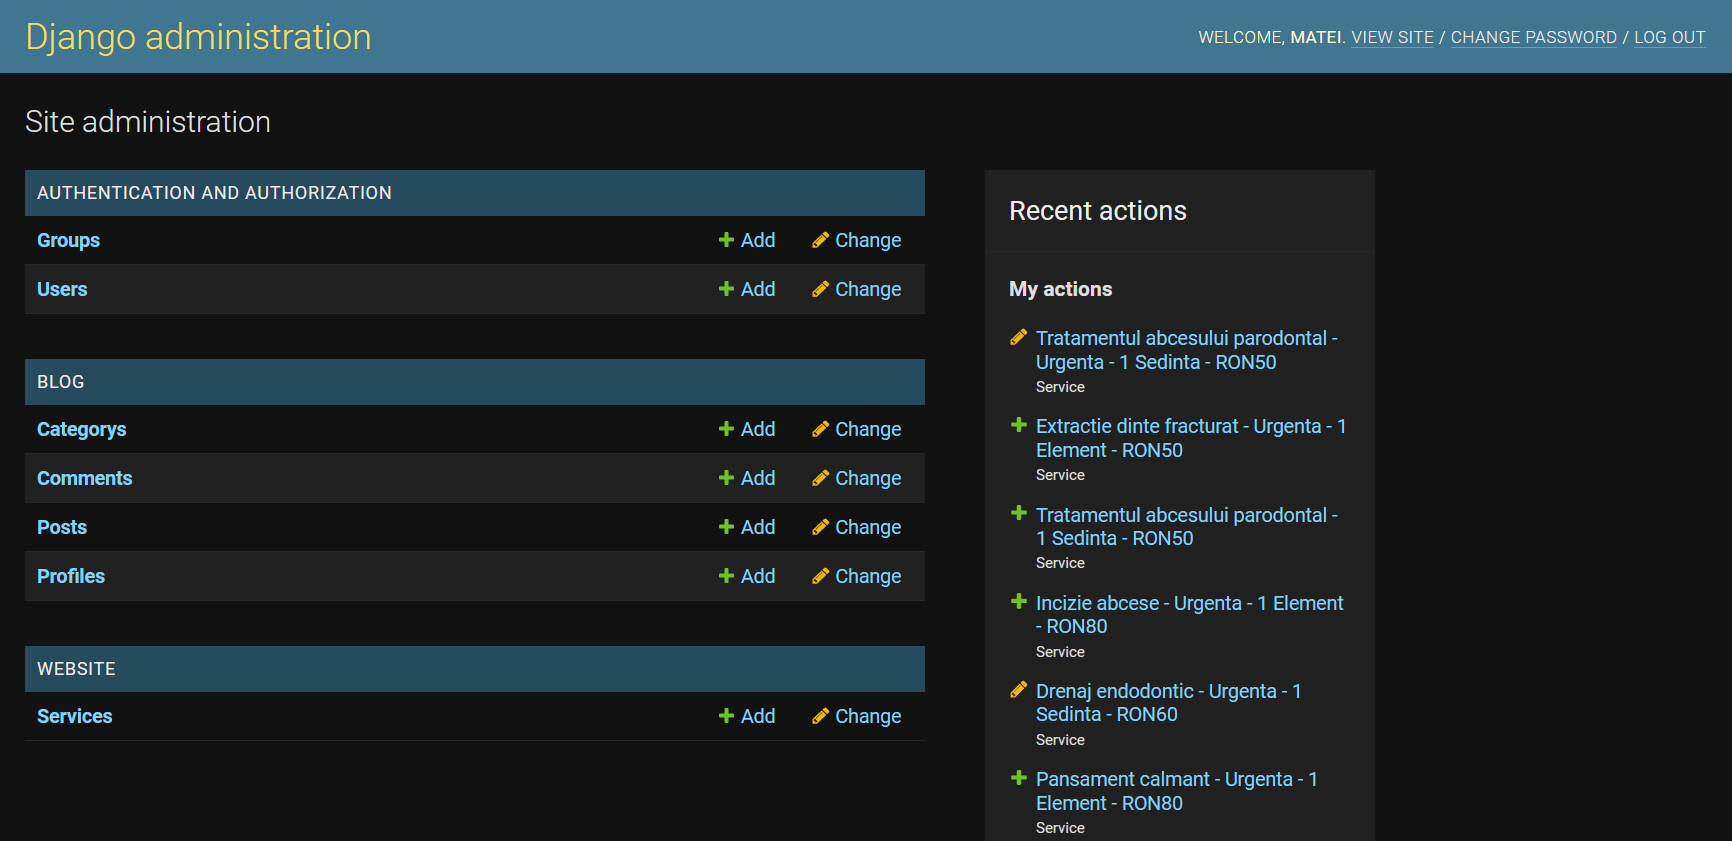
\includegraphics[width=0.8\columnwidth]{Django_admin.png} % Example image
	\caption{The Django admin site}
	\label{fig:djadmin}
\end{figure}

%------------------------------------------------

\subsubsection{Staff și Utilizatori}



Secțiunea adminintrativă Fig.\ref{fig:staff&users}, folosită pentru gestionare utilizatorilor, ne oferă lista completă a profilelor celor care access pe site. Aici putem sa verificăm tipul de access, datele personale și alte informații legate de utilizatori. Trebuie mentionat ca nu toți utilizatorii au același privilegii: cei care fac parte din staff au access la sectiunea administrativă, restul având access numai pe pagina de blog. \\
Tot din aceasta zonă putem sa adaugam un nou utilizator, să stergem un utilizator existent sau să modificăm informațiile sau tipul de access al unui utilizator existent. Este de mentionat că în această secțiune, numai personalul administrativ are access și modificările conturilor ar trebui facute în această secțiune numai dacă există motive întemeiate. Altfe, este disponibilă o pagina din blog pentru ca utilizatorii să își poată gestiona singuri conturile.

\begin{figure}[h] % [h] forces the figure to be output where it is defined in the code (it suppresses floating)
	\centering
	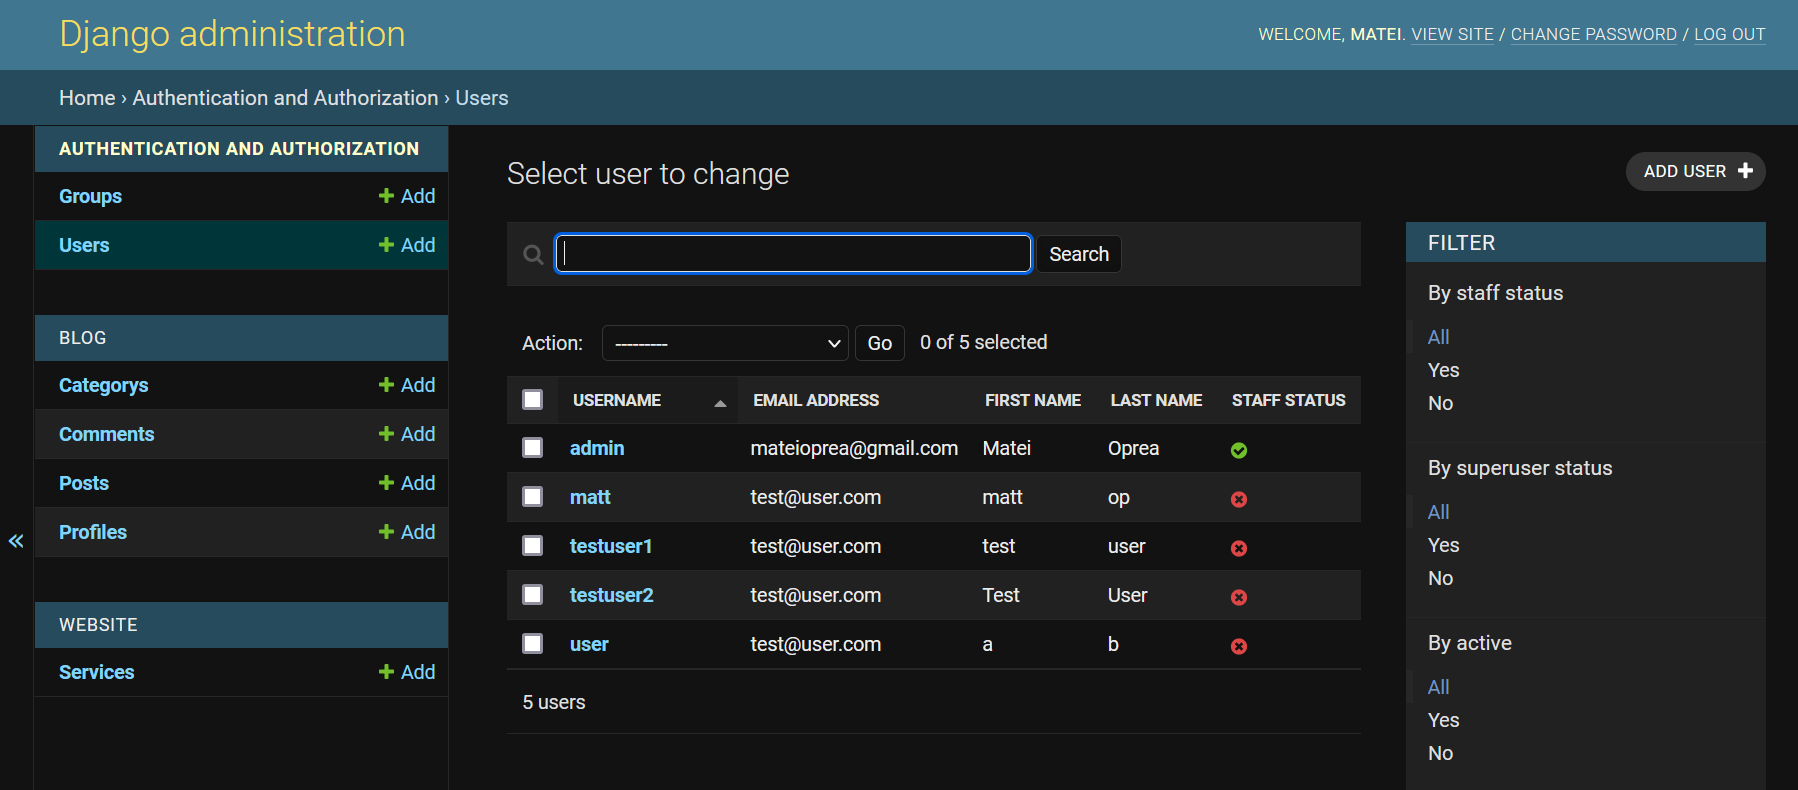
\includegraphics[width=0.8\columnwidth]{Staff_users.png} % Example image
	\caption{Staff si Utilizatori}
	\label{fig:staff&users}
\end{figure}

%------------------------------------------------

\subsubsection{Gestionare Bază de Date}

Tot în secțiunea administrativă avem posibilitatea să vedem conținutul bazei de date Fig.\ref{fig:dbadmin}, pentru modelele care au fost înregistrate în aplicația admin. Aici putem să accesăm direct datele conținute de  tabele, să le modificăm, să le ștergem sau să adăugam noi articole. Aceiași mențiune se aplică și aici, ca în cazul celorlalte view-uri ale administratiei, și anume că această interfață nu este cea utiliztă în mod uzual pentru a adăuga conțiunut, ci este rezervată administrației pentru a interveni sau a modifica date în caz de necesitate.

\begin{figure}[h] % [h] forces the figure to be output where it is defined in the code (it suppresses floating)
	\centering
	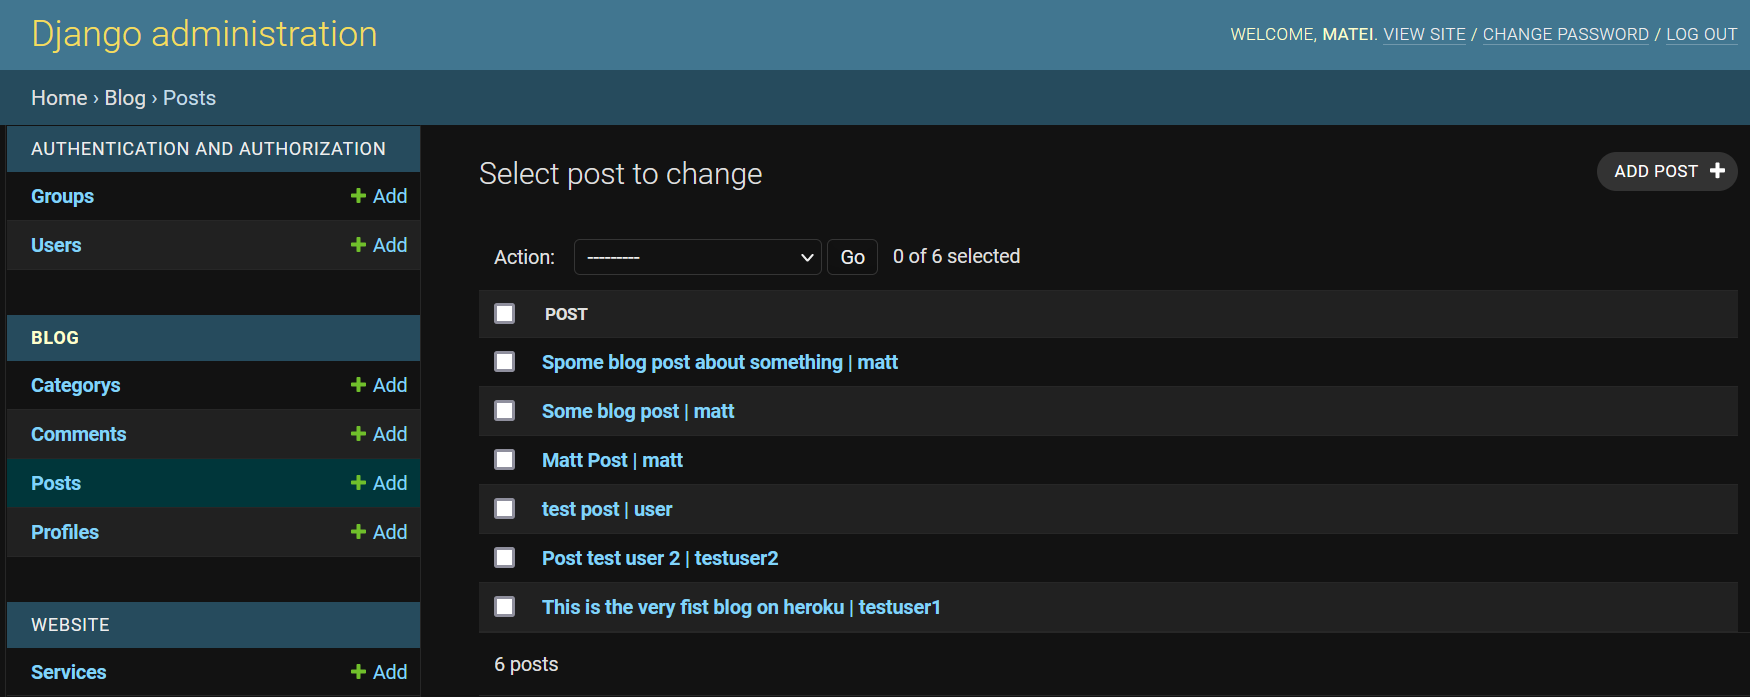
\includegraphics[width=0.8\columnwidth]{Database_admin.png} % Example image
	\caption{Admin Database View}
	\label{fig:dbadmin}
\end{figure}

Figura \ref{fig:dbstruct} arată cum este structurată baza de date folosita în această aplicatie. Baza de date a fost inițial dezvoltată în SqLite, ulterior fiind schimbată la PostgreSQL pentru a putea fii folosită pe serverul de hoasting. 

\begin{figure}[h] % [h] forces the figure to be output where it is defined in the code (it suppresses floating)
	\centering
	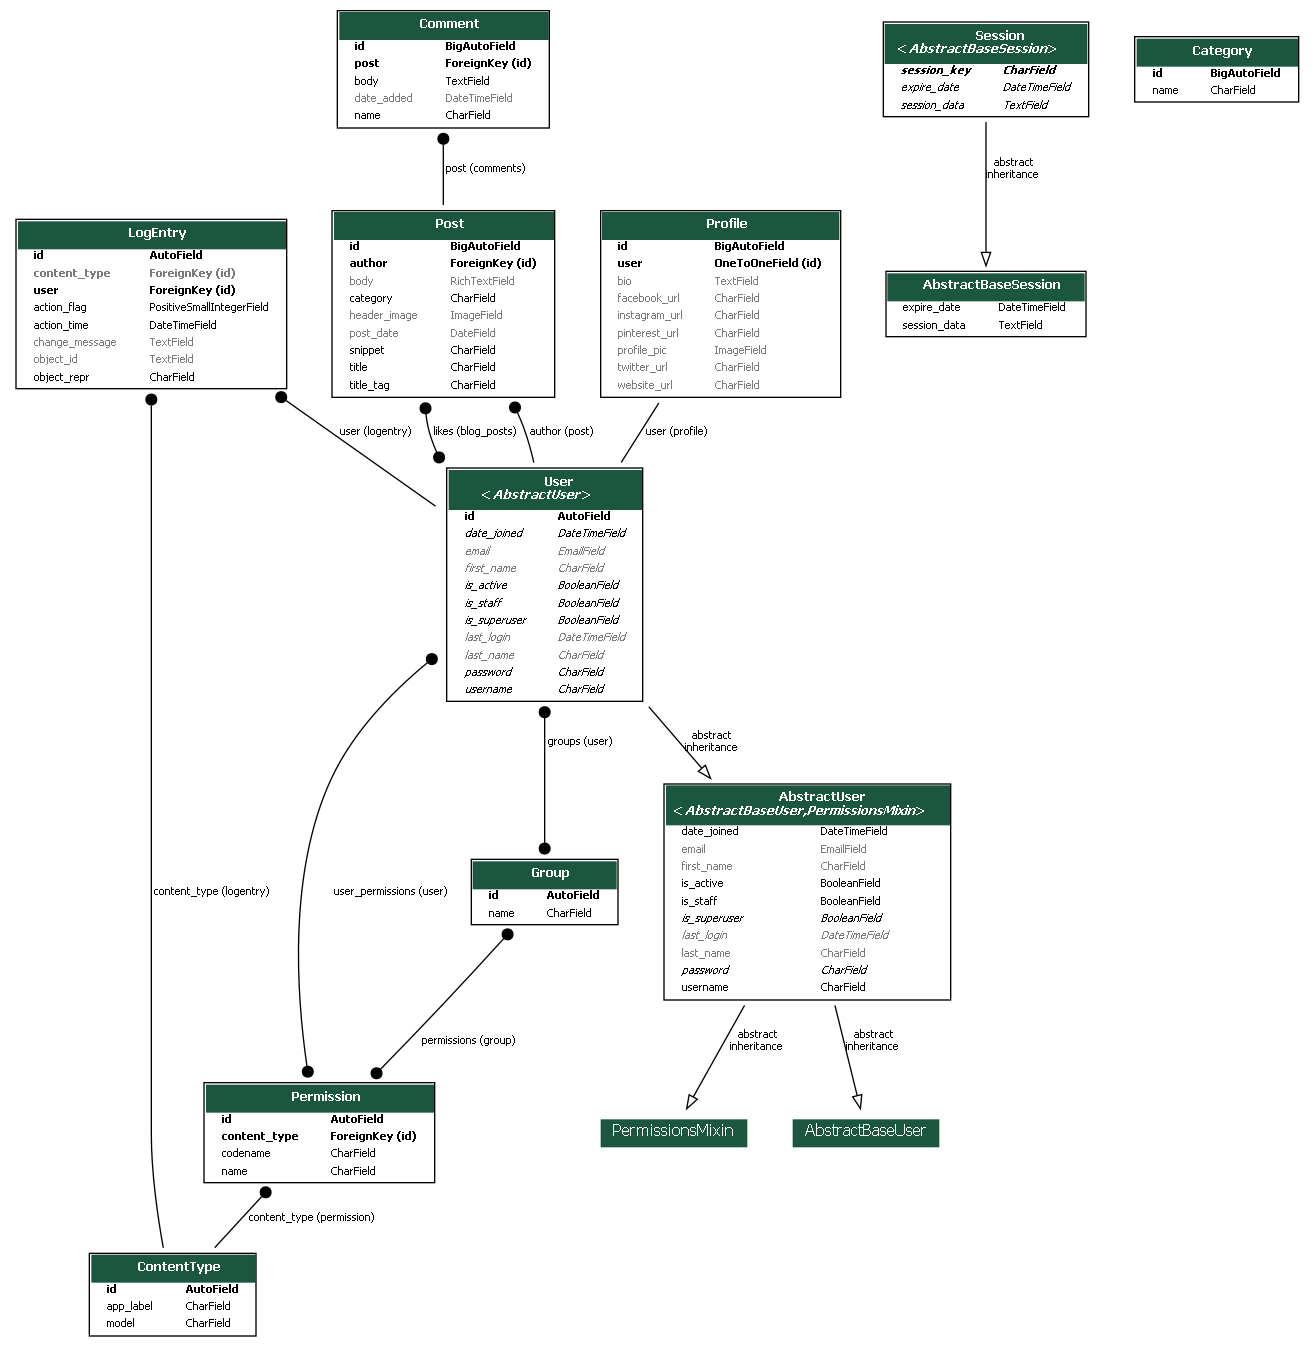
\includegraphics[width=0.8\columnwidth]{my_project_visualized.png} % Example image
	\caption{Structură Bază Date}
	\label{fig:dbstruct}
\end{figure}
%------------------------------------------------

\subsection{Web-site}

Partea de Web-site efectiv a aplicației a fost realizată cu un template \footnote{https://colorlib.com/} gratuit. Acesta este format din pagini HTML împreună cu JavaScript pentru a realiza efectele vizuale dorite. Infomațiile oferite de Site au fost actualizate pentru a reflecta imaginea cabinetului B-Wise Dental.

%------------------------------------------------

\subsubsection{Prezentare Cabinet}

Prezentarea Cabinetului este realizată în trei secțiuni. Pagina de start (acasă) \footnote{https://first-dental-website.herokuapp.com/} are un sumar cuprinzător ce conține: deviza cabinetului, informații legate de experiența și serviciile oferite, o lista scurtă de prețuri și un formular de contact pentru programări. Acesta din urmă va fi discutat pe larg în ultima parte a acestei sectiuni.\\
Informațiile legate de experiență și echipă sunt prezentate din nou în secțiunea "despre" a site-ului. Iar în secțiunea "servicii", Fig.\ref{fig:serv_details}, găsim o descriere detaliata a serviciilor oferite de cabinet. 

\begin{figure}[h] % [h] forces the figure to be output where it is defined in the code (it suppresses floating)
	\centering
	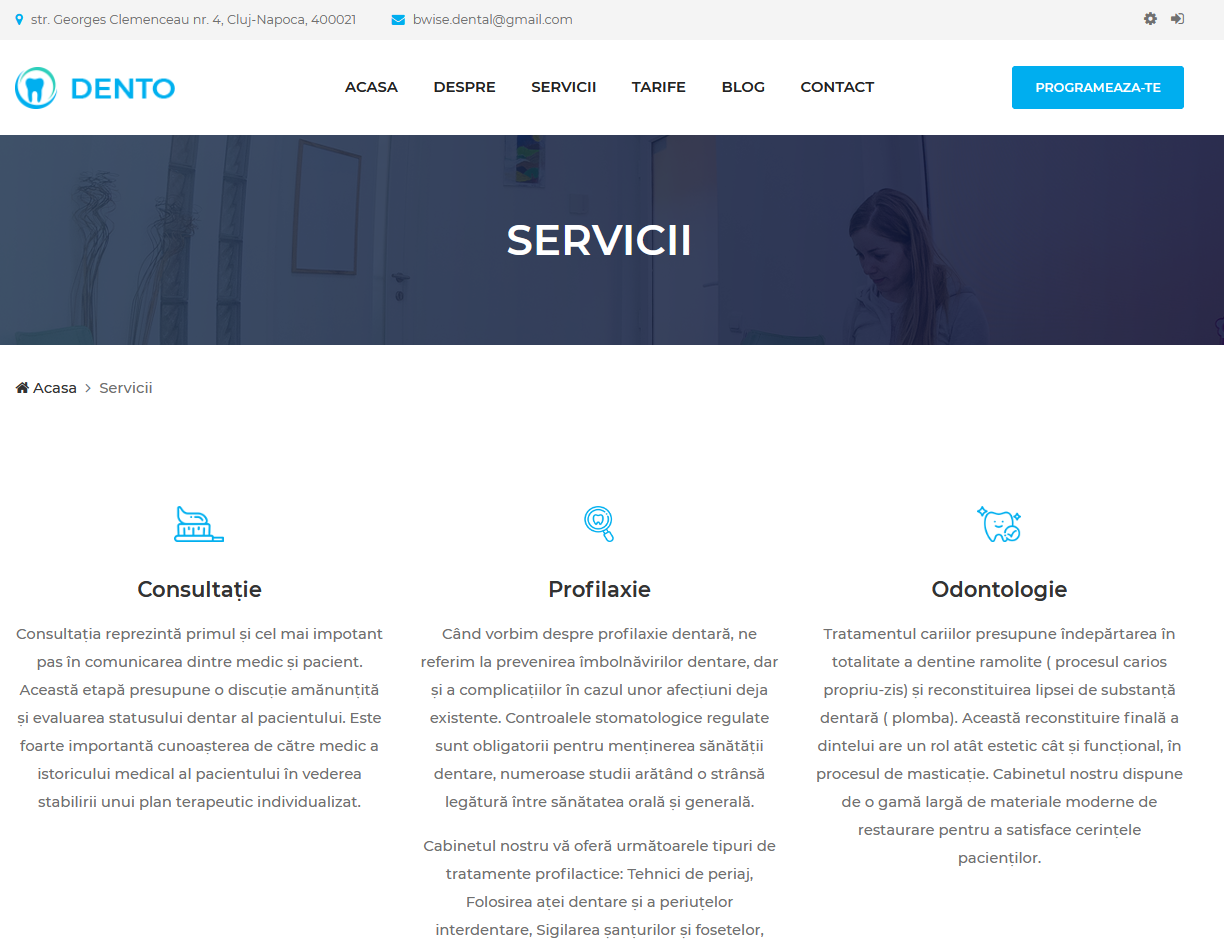
\includegraphics[width=0.8\columnwidth]{Servicii_details.png} % Example image
	\caption{Pagina de prezentare a serviciilor oferite}
	\label{fig:serv_details}
\end{figure}


%------------------------------------------------

\subsubsection{Listă Prețuri}

În secțiunea "Tarife" sunt prezentate costurile aferente serviciilor Fig.\ref{fig:serv_site} . Ca utilitate oferită de aceast site, detaliile legate de numele serviciului, costul sau în câte etape se realizează serviciul, pot fi modificate din sectiune "admin" Fig.\ref{fig:serv_admin}, cu ajutorul unui cont de staff. Aceasta ușurează mentenanța site-ului și poate fi realizată independent de serviciul de hoasting și fară a modifica pagina HTML. 

\begin{figure}[h] % [h] forces the figure to be output where it is defined in the code (it suppresses floating)
	\centering
	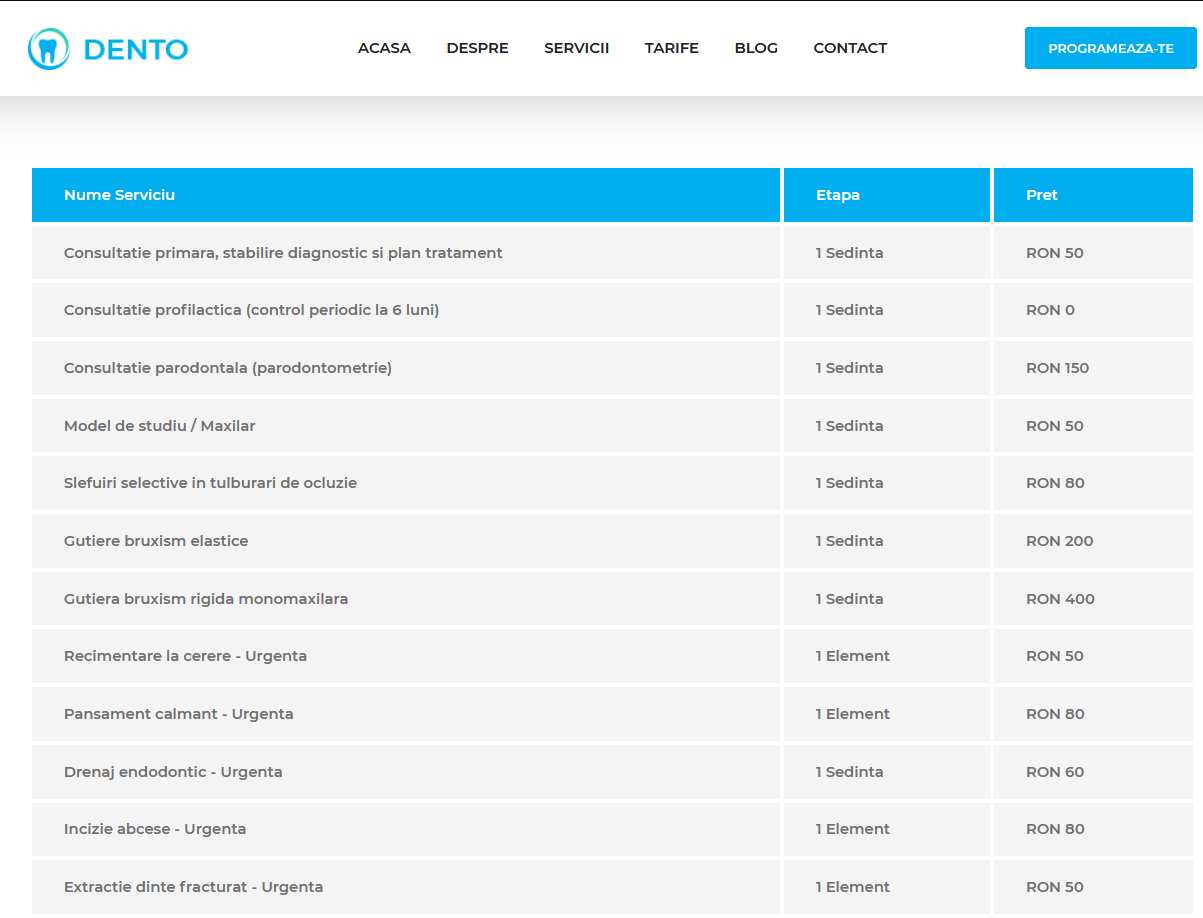
\includegraphics[width=0.8\columnwidth]{Servicii_site.png} % Example image
	\caption{Prezentarea tarifelor}
	\label{fig:serv_site}
\end{figure}

\begin{figure}[h] % [h] forces the figure to be output where it is defined in the code (it suppresses floating)
	\centering
	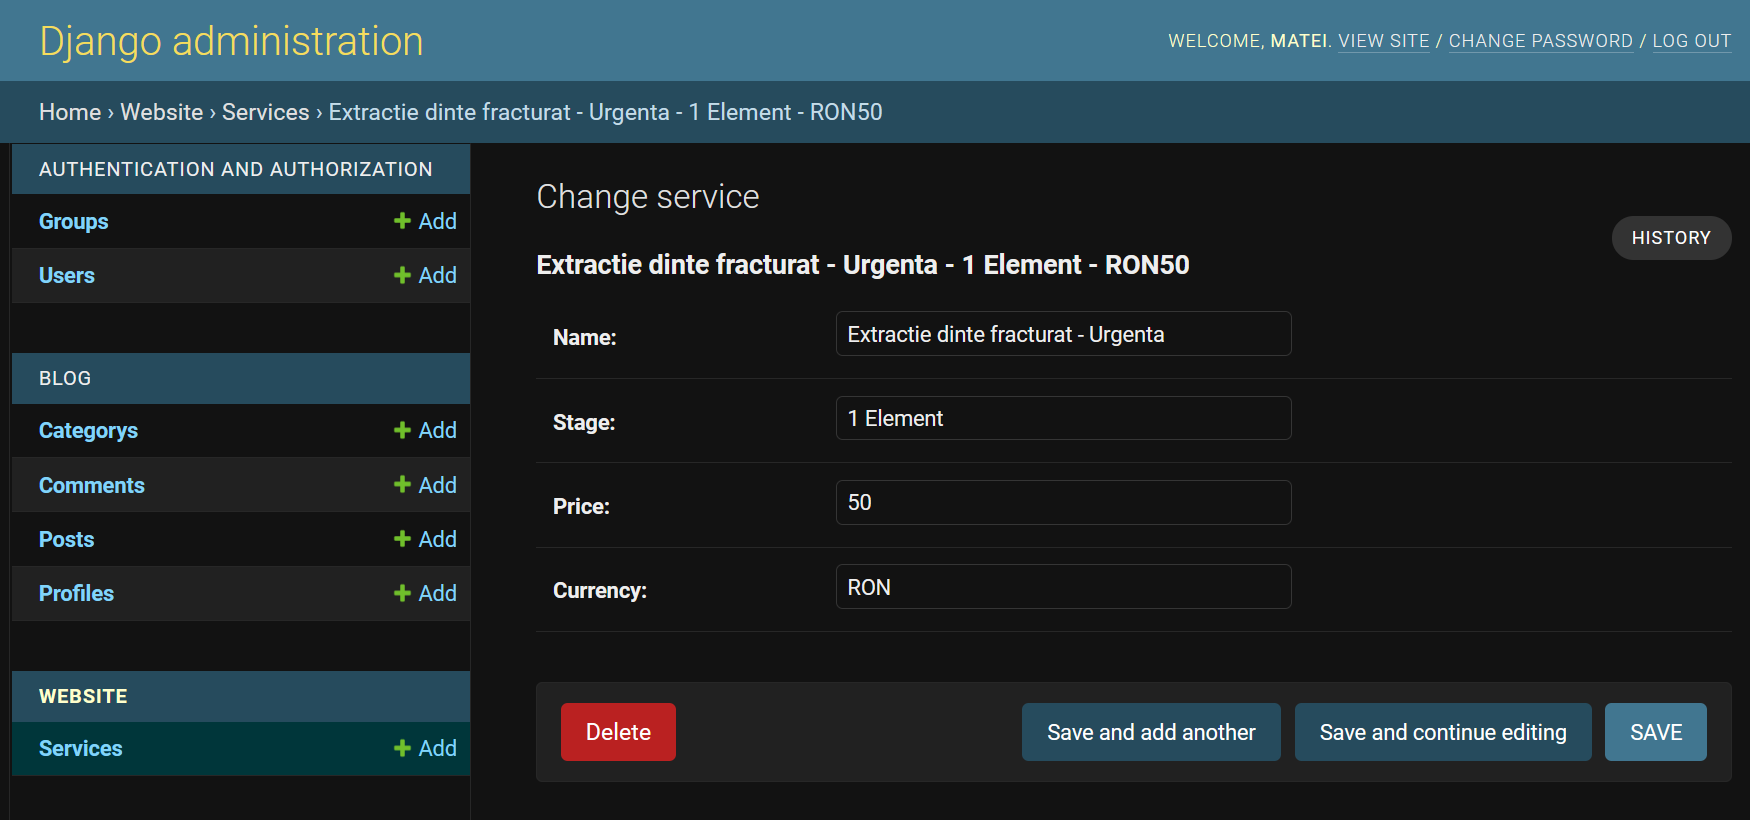
\includegraphics[width=0.8\columnwidth]{Servicii_admin.png} % Example image
	\caption{Posibilitatea de a gestiona informațiile prezentate in secțiunea "Tarife" din zona de administrație}
	\label{fig:serv_admin}
\end{figure}


%------------------------------------------------

\subsubsection{Programare și Contact}

Pentru a facilita contactul cu clienții, sunt disponibilile două formulare de contact. Unul presentat în Fig.\ref{fig:form_prog} destinat realizării unei programări pentru consult. Programare care va fi confirmată ulterior telefonic de către secretara cabinetului. Și un al doilea formular prezentat in Fig.\ref{fig:form_contact} care este destinat trimiterii unui mesaj către cabinet. Tot aici este intgrat un iframe goolge maps pentru a ușura gasirea locației cabinetului.\\
Automatizarea mesajelor este realizată în spate cu ajutorul serverului gmail, care va expedia mesajele trimise de pe site către adresa cabinetului. Din motive de securitate, toate detallile legate de comunicare cu serverul de mail vor fi stocate ca variablile de mediu și se va evita salvarea de date ce pot compromite accesul la serviciul de mail direct în codul uplodat pe serverul de host sau git repository.

\lstinputlisting[
	caption=Gmail mail server set-up, % Caption above the listing
	label=lst:gmail_conf, % Label for referencing this listing
	language=Python, % Use Perl functions/syntax highlighting
	frame=single, % Frame around the code listing
	showstringspaces=false, % Don't put marks in string spaces
	numbers=left, % Line numbers on left
	numberstyle=\tiny, % Line numbers styling
	]{conf_mail.py}
 

\begin{figure}[h] % [h] forces the figure to be output where it is defined in the code (it suppresses floating)
	\centering
	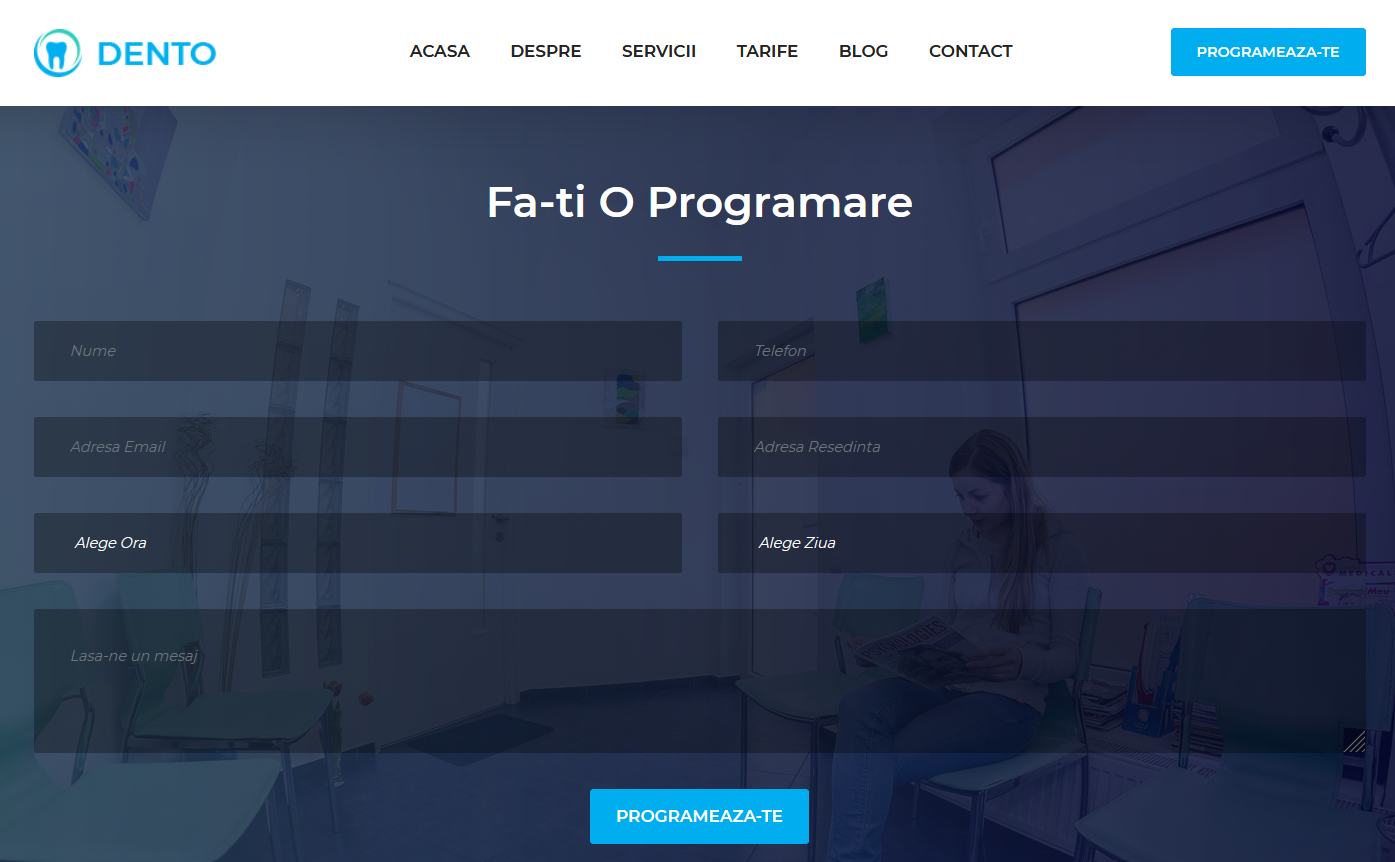
\includegraphics[width=0.8\columnwidth]{form_programare.png} % Example image
	\caption{Formular de programare pentru consult}
	\label{fig:form_prog}
\end{figure}

\begin{figure}[h] % [h] forces the figure to be output where it is defined in the code (it suppresses floating)
	\centering
	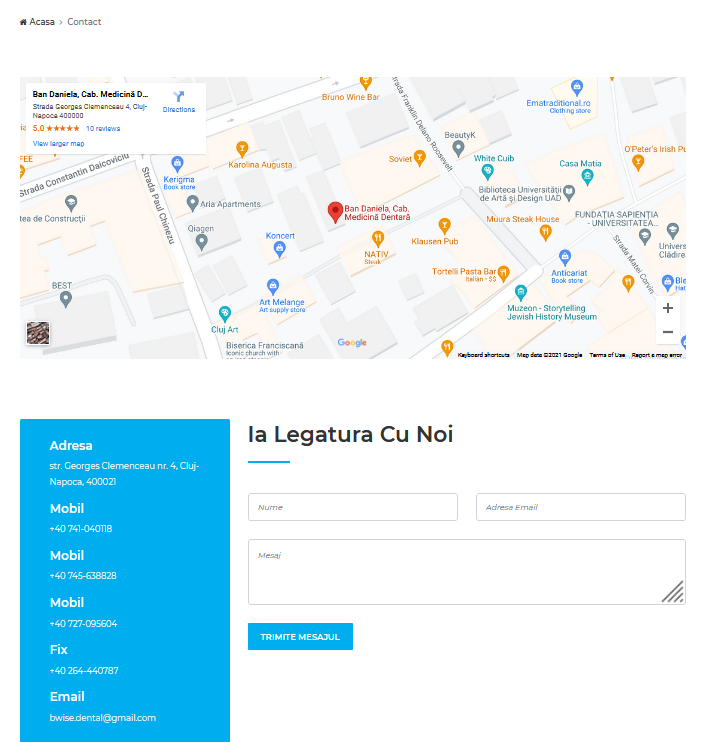
\includegraphics[width=0.8\columnwidth]{form_contact.png} % Example image
	\caption{Posibilitatea de a trimite un mesaj cabinetului în secțiunea contact}
	\label{fig:form_contact}
\end{figure}

%------------------------------------------------



\subsection{Blog}

%------------------------------------------------

\subsubsection{Creare și Înregistrare Utilizator}

%------------------------------------------------

\subsubsection{Create, Editare, Stergere Articol Blog}

%------------------------------------------------

\subsubsection{Comentare Articol}

%------------------------------------------------


\begin{comment}
\section{Understanding Text}

\subsection{How much wood would a woodchuck chuck if a woodchuck could chuck wood?}

%------------------------------------------------

\subsubsection{Suppose ``chuck" implies throwing.}

According to the Associated Press (1988), a New York Fish and Wildlife technician named Richard Thomas calculated the volume of dirt in a typical 25--30 foot (7.6--9.1 m) long woodchuck burrow and had determined that if the woodchuck had moved an equivalent volume of wood, it could move ``about \textbf{700 pounds (320 kg)} on a good day, with the wind at his back".

%------------------------------------------------

\subsubsection{Suppose ``chuck" implies vomiting.}

A woodchuck can ingest 361.92 cm\textsuperscript{3} (22.09 cu in) of wood per day. Assuming immediate expulsion on ingestion with a 5\% retainment rate, a woodchuck could chuck \textbf{343.82 cm\textsuperscript{3}} of wood per day.

%------------------------------------------------

\paragraph{Bonus: suppose there is no woodchuck.}

Fusce varius orci ac magna dapibus porttitor. In tempor leo a neque bibendum sollicitudin. Nulla pretium fermentum nisi, eget sodales magna facilisis eu. Praesent aliquet nulla ut bibendum lacinia. Donec vel mauris vulputate, commodo ligula ut, egestas orci. Suspendisse commodo odio sed hendrerit lobortis. Donec finibus eros erat, vel ornare enim mattis et.

%----------------------------------------------------------------------------------------
%	EQUATION EXAMPLES
%----------------------------------------------------------------------------------------

\section{Interpreting Equations}

\subsection{Identify the author of Equation \ref{eq:bayes} below and briefly describe it in English.}

\begin{align} 
	\label{eq:bayes}
	\begin{split}
		P(A|B) = \frac{P(B|A)P(A)}{P(B)}
	\end{split}					
\end{align}

Lorem ipsum dolor sit amet, consectetur adipiscing elit. Praesent porttitor arcu luctus, imperdiet urna iaculis, mattis eros. Pellentesque iaculis odio vel nisl ullamcorper, nec faucibus ipsum molestie. Sed dictum nisl non aliquet porttitor. Etiam vulputate arcu dignissim, finibus sem et, viverra nisl. Aenean luctus congue massa, ut laoreet metus ornare in. Nunc fermentum nisi imperdiet lectus tincidunt vestibulum at ac elit. Nulla mattis nisl eu malesuada suscipit.

%------------------------------------------------

\subsection{Try to make sense of some more equations.}

\begin{align} 
	\begin{split}
		(x+y)^3 &= (x+y)^2(x+y)\\
		&=(x^2+2xy+y^2)(x+y)\\
		&=(x^3+2x^2y+xy^2) + (x^2y+2xy^2+y^3)\\
		&=x^3+3x^2y+3xy^2+y^3
	\end{split}					
\end{align}

Lorem ipsum dolor sit amet, consectetuer adipiscing elit. 
\begin{align}
	A = 
	\begin{bmatrix}
		A_{11} & A_{21} \\
		A_{21} & A_{22}
	\end{bmatrix}
\end{align}
Aenean commodo ligula eget dolor. Aenean massa. Cum sociis natoque penatibus et magnis dis parturient montes, nascetur ridiculus mus. Donec quam felis, ultricies nec, pellentesque eu, pretium quis, sem.

%----------------------------------------------------------------------------------------
%	LIST EXAMPLES
%----------------------------------------------------------------------------------------

\section{Viewing Lists}

\subsection{Bullet Point List}

\begin{itemize}
	\item First item in a list 
		\begin{itemize}
		\item First item in a list 
			\begin{itemize}
			\item First item in a list 
			\item Second item in a list 
			\end{itemize}
		\item Second item in a list 
		\end{itemize}
	\item Second item in a list 
\end{itemize}

%------------------------------------------------

\subsection{Numbered List}

\begin{enumerate}
	\item First item in a list 
	\item Second item in a list 
	\item Third item in a list
\end{enumerate}

%----------------------------------------------------------------------------------------
%	TABLE EXAMPLE
%----------------------------------------------------------------------------------------

\section{Interpreting a Table}

\begin{table}[h] % [h] forces the table to be output where it is defined in the code (it suppresses floating)
	\centering % Centre the table
	\begin{tabular}{l l l}
		\toprule
		\textit{Per 50g} & \textbf{Pork} & \textbf{Soy} \\
		\midrule
		Energy & 760kJ & 538kJ\\
		Protein & 7.0g & 9.3g\\
		Carbohydrate & 0.0g & 4.9g\\
		Fat & 16.8g & 9.1g\\
		Sodium & 0.4g & 0.4g\\
		Fibre & 0.0g & 1.4g\\
		\bottomrule
	\end{tabular}
	\caption{Sausage nutrition.}
\end{table}

%------------------------------------------------

\subsection{The table above shows the nutritional consistencies of two sausage types. Explain their relative differences given what you know about daily adult nutritional recommendations.}

Lorem ipsum dolor sit amet, consectetur adipiscing elit. Praesent porttitor arcu luctus, imperdiet urna iaculis, mattis eros. Pellentesque iaculis odio vel nisl ullamcorper, nec faucibus ipsum molestie. Sed dictum nisl non aliquet porttitor. Etiam vulputate arcu dignissim, finibus sem et, viverra nisl. Aenean luctus congue massa, ut laoreet metus ornare in. Nunc fermentum nisi imperdiet lectus tincidunt vestibulum at ac elit. Nulla mattis nisl eu malesuada suscipit.

%----------------------------------------------------------------------------------------
%	CODE LISTING EXAMPLE
%----------------------------------------------------------------------------------------

\section{Reading a Code Listing}

\lstinputlisting[
	caption=Luftballons Perl Script., % Caption above the listing
	label=lst:luftballons, % Label for referencing this listing
	language=Perl, % Use Perl functions/syntax highlighting
	frame=single, % Frame around the code listing
	showstringspaces=false, % Don't put marks in string spaces
	numbers=left, % Line numbers on left
	numberstyle=\tiny, % Line numbers styling
	]{luftballons.pl}

%------------------------------------------------

\subsection{How many luftballons will be output by the Listing \ref{lst:luftballons} above?}

Aliquam arcu turpis, ultrices sed luctus ac, vehicula id metus. Morbi eu feugiat velit, et tempus augue. Proin ac mattis tortor. Donec tincidunt, ante rhoncus luctus semper, arcu lorem lobortis justo, nec convallis ante quam quis lectus. Aenean tincidunt sodales massa, et hendrerit tellus mattis ac. Sed non pretium nibh. Donec cursus maximus luctus. Vivamus lobortis eros et massa porta porttitor.

%------------------------------------------------

\subsection{Identify the regular expression in Listing \ref{lst:luftballons} and explain how it relates to the anti-war sentiments found in the rest of the script.}

Fusce varius orci ac magna dapibus porttitor. In tempor leo a neque bibendum sollicitudin. Nulla pretium fermentum nisi, eget sodales magna facilisis eu. Praesent aliquet nulla ut bibendum lacinia. Donec vel mauris vulputate, commodo ligula ut, egestas orci. Suspendisse commodo odio sed hendrerit lobortis. Donec finibus eros erat, vel ornare enim mattis et.

%----------------------------------------------------------------------------------------
\end{comment}
\end{document}
